% Kompilasi: xelatex main; bibtex main; xelatex main; xelatex main  (lihat README.md)
\documentclass[11pt,a4paper]{article}

\usepackage{fontspec}
\usepackage[margin=2.5cm]{geometry}
\usepackage{booktabs,tabularx,array}
\usepackage{graphicx}
\usepackage{xcolor}
\usepackage{caption}
\usepackage[authoryear,round]{natbib}
\usepackage[colorlinks=true,linkcolor=blue!50!black,citecolor=blue!50!black,urlcolor=blue!50!black]{hyperref}
\usepackage{setspace}
\onehalfspacing

\newcolumntype{Y}{>{\raggedright\arraybackslash}X}
% Penanda pekerjaan yang belum selesai (merah). Hapus semua \todo sebelum submit.
\newcommand{\todo}[1]{\textcolor{red}{[#1]}}

\title{Mapping the Thematic Structure and Emerging Trends of Large Language Model Research Across Multi-Agent Systems, On-Device Deployment, and Inventory Management: A Bibliometric Analysis}
\author{Aldian Yohanes\thanks{Faculty of Information Technology, Universitas Tarumanagara, Jakarta, Indonesia. \todo{co-authors, supervisor, e-mail}}}
\date{\todo{date}}

\begin{document}
\maketitle

\begin{abstract}
\noindent
\textbf{Background.} Research on large language models (LLMs) has grown quickly, but it is spread over separate streams, such as LLM-based agents, models that run on the device or in the browser, and applications in inventory management for small businesses.
\textbf{Aim.} This study maps how these three streams are structured, and where they connect, using bibliometric methods.
\textbf{Data.} We analyse 485 journal articles published between 2023 and 2026, retrieved from OpenAlex on 28 October 2026 and screened with language-model assistance.
\textbf{Methods.} We combine performance analysis, bibliographic coupling, co-citation analysis, and co-word analysis.
\textbf{Findings.} Co-word analysis yields three clusters: one around agents, retrieval-augmented generation, and business applications, and two around edge deployment and small language models. The business-oriented cluster is loosely separated from the edge clusters in all 63 robustness runs, but about a fifth to a half of the link weight crosses clusters. In the co-citation network, the business-related stream is reduced to a group of four references on generative AI in supply chains, while efficient-inference work dominates the foundations of the field.
\textbf{Contribution.} The study provides a first science map across these streams, shows that evidence on LLMs for inventory management is thin, and sets out a research agenda. \todo{check the claims against the final screened dataset and the manual validation}
\end{abstract}

\noindent\textbf{Keywords:} large language models; multi-agent systems; on-device inference; inventory management; bibliometric analysis; science mapping

\section{Introduction}

% Setiap sitasi diambil dari OpenAlex dan kalimatnya dicocokkan dengan abstrak sumbernya (analysis/Skrip/ambil_rujukan.py,
% analysis/Hasil/abstrak_rujukan.json). Klaim tanpa sumber ditandai \todo.

Large language models (LLMs) build on the Transformer architecture \parencite{vaswani2017}. \textcite{brown2020} showed that a single model can handle many language tasks from only a few examples, and the release of open models \parencite{touvron2023} made it practical to run them outside large data centres. Deployment is therefore no longer tied to the cloud. Models now run at the edge of the network, on phones, and inside web browsers; WebLLM, for instance, performs inference entirely in the browser through WebGPU \parencite{ruan2024webllm}.

Research on these models appears to have divided into streams that seldom cite one another. One stream studies LLM-based autonomous agents \parencite{wang2024agents}. A second asks how language models can run on resource-constrained devices and has produced surveys of edge and mobile-edge LLMs \parencite{friha2024,qu2025,zheng2025} and of small language models \parencite{wang2025slm}. A third applies generative AI and LLMs to operations and supply chains, including inventory management and demand forecasting \parencite{jackson2024,nakhost2025,wamba2023}. Small businesses are a setting in which all three streams could meet, because they often have limited cloud budgets and sensitive data \todo{cite evidence on cloud costs and data sensitivity in small businesses}. Whether the literature connects the streams is not yet clear.

Existing reviews cover one stream at a time. The edge-LLM surveys deal with architectures, optimisation, and deployment techniques \parencite{friha2024,qu2025,zheng2025}. The agent survey explains how agents are built and where they are applied \parencite{wang2024agents}. The supply chain studies examine the capabilities and perceived benefits of generative AI in operations \parencite{jackson2024,wamba2023}, and a related review addresses explainable AI \parencite{kosasih2023}. Bibliometric work on LLMs does exist, but it is either broad, with over 5,000 publications up to early 2023 \parencite{fan2024}, or tied to a single domain such as transportation \parencite{hassan2025}. A bibliometric review of agentic AI in small, medium, and micro enterprises reports a sharp rise since 2022 driven by LLMs and multi-agent systems \parencite{olujimi2025}, yet it leaves out the on-device stream. \todo{recheck in Scopus and Web of Science for earlier bibliometric studies that join the three streams; this search was done only in OpenAlex}

A bibliometric analysis suits this problem because it describes the structure of a fast-growing field and shows where its streams connect or stay apart \parencite{donthu2021,zupic2015}. This study maps the journal literature of 2023 to 2026 across the three streams and asks three questions. RQ1: who and what shaped research on LLMs across agents, on-device deployment, and inventory management (citation analysis)? RQ2: what are the foundations and the current research streams (co-citation analysis and bibliographic coupling)? RQ3: which concepts and gaps are emerging (co-word analysis)? \todo{state the theoretical, methodological, practical, and policy contributions once the discussion is final}

\section{Methodology}

\subsection{Bibliometric approach}
Bibliometric analysis is a quantitative method that studies bibliographic data through performance analysis and science mapping \citep{donthu2021,zupic2015}. We used performance analysis, bibliographic coupling, co-citation analysis, and co-word analysis, so that the field is described from its foundations (co-citation), its current streams (coupling), and its concepts (co-word).

\subsection{Research design and data collection}
We retrieved records from OpenAlex through its public interface on 28 October 2026. \todo{cite the OpenAlex paper after verification: arXiv 2205.01833 was not verified} The search covered titles and abstracts, was limited to document type ``article'', and covered publication years 2023 to 2026 (2026 is a partial year). OpenAlex was chosen because it is open and the queries can be repeated. We did not use Scopus or Web of Science, which are the databases named in most bibliometric guidance \citep{donthu2021}; \citet{zhu2020}, \citet{mongeon2016}, and \citet{echchakoui2020} discuss the choice between them. The consequences for coverage are discussed in Section~\ref{sec:limitations}.

Three search blocks represent the three streams (Table~\ref{tab:search}). Terms within a concept block are joined with OR, and blocks are joined with AND. In block C, the exclusion of stock-market terms removes records where ``stock'' refers to share prices.

\begin{table}[htbp]
\centering
\small
\caption{Search blocks (keywords and justification). LLM terms: ``large language model'', LLM, LLMs. LM terms: LLM terms plus ``small language model'' and SLM.}
\label{tab:search}
\begin{tabularx}{\textwidth}{lYY}
\toprule
\textbf{Block} & \textbf{Search string} & \textbf{Justification} \\
\midrule
A & LLM terms AND (``multi-agent'' OR multiagent OR agentic OR ``LLM agent'' OR ``LLM agents'') AND (``inventory management'' OR ``inventory control'' OR ``supply chain management'' OR SME OR SMEs OR ``small business'' OR ``small businesses'' OR retail OR MSME OR ``business process'') & Multi-agent and agentic LLM work in operational or business settings \\
B & LM terms AND (WebLLM OR WebGPU OR ``in-browser'' OR ``browser-based'' OR ``on-device'' OR ``edge device'' OR ``edge devices'') & Language models that run in the browser, on the device, or at the edge \\
C & LM terms AND (inventory OR stock) AND (retail OR SME OR SMEs OR ``small business'' OR ``small businesses'' OR MSME OR warehouse OR ``supply chain management'' OR procurement OR ``demand forecasting'' OR ``sales forecasting'' OR replenishment OR ``point of sale'' OR e-commerce) NOT (``stock market'' OR ``stock price'' OR ``stock prices'' OR ``stock exchange'' OR ``stock trading'' OR ``stock returns'') & Language-model work on inventory, stock, and demand in business settings \\
\bottomrule
\end{tabularx}
\end{table}

\subsection{Screening and final dataset}
The three blocks returned 149, 584, and 87 records (820 in total), which formed 801 unique records. We removed 16 records that shared a normalised title with another record, keeping the version with a journal source, reference data, and a DOI. We then excluded 77 records hosted on Zenodo, because it is a repository without a guaranteed peer-review process. The remaining 708 records were screened on title and abstract.

Screening was assisted by language models in two passes. In the first pass, eight Claude Haiku instances judged about 89 records each as relevant, not relevant, or uncertain. A record was relevant when a language model and at least one of the three topics were a main or important part of the work. This pass gave 430 relevant, 150 not relevant, and 128 uncertain records. In the second pass, three Claude Sonnet instances re-judged the 128 uncertain records with longer abstracts and a confidence level, resolving 55 as relevant and 72 as not relevant, and leaving one uncertain. The final dataset has \textbf{485 records} (Figure~\ref{fig:prisma}). \todo{human validation: report agreement on the 20-record sample; 97 of 128 second-pass decisions had low model confidence}

\begin{figure}[htbp]
\centering
\fbox{\parbox{0.9\textwidth}{\centering\small
820 records retrieved $\rightarrow$ 801 unique $\rightarrow$ 785 after title de-duplication $\rightarrow$ 708 after excluding Zenodo $\rightarrow$ 485 included (222 excluded, 1 unresolved)}}
\caption{Record flow (PRISMA-style counts). \todo{replace with a proper flow diagram}}
\label{fig:prisma}
\end{figure}

\subsection{Analysis}
Performance analysis counted publications per year, source, country (author affiliations), and author, together with citations. For science mapping we used two techniques \citep{donthu2021,zupic2015}:
\begin{itemize}
  \item \textbf{Co-word analysis} used the keywords assigned by OpenAlex. Synonyms were merged (for example ``LLM'' and ``large language models''), and ``large language model'' and ``artificial intelligence'' were removed because they occur in nearly all records. We kept keywords with at least eight occurrences (68 keywords).
  \item \textbf{Bibliographic coupling and co-citation} used reference lists. OpenAlex had reference data for 255 of the 485 records; we added Crossref data through DOIs, which brought the total to 278 records (57.3\%). Two records were linked when they shared at least two references. For co-citation we kept references cited by at least three records in the dataset and removed eight items that were data artefacts: proceedings volumes, which are not single works, and one reference that was cited by 22 edge-LLM papers although its title concerns intelligent tutoring systems (a suspected linking error in OpenAlex, not verified).
\end{itemize}
Clusters were found with the Louvain algorithm \citep{blondel2008}, computed in Python (networkx, fixed random seed) and displayed with VOSviewer 1.6.21 \citep{vaneck2010} through its map and network file formats. The cluster membership in the figures is therefore the one computed in Python. To test robustness, we repeated the co-word clustering with minimum occurrences of 5, 8, and 12, with 20 random seeds, and with a greedy modularity algorithm. The target of 200 to 1{,}000 records follows the sample-size guidance attributed to \citet{rogers2020} \todo{read the paper to confirm the range}; the record flow follows the PRISMA statement \citep{page2021}.

\section{Findings and discussion}

\subsection{Publication and citation trends (RQ1)}
The dataset has 485 articles. Output grows quickly: 4 articles in 2023, 37 in 2024, 151 in 2025, and 293 in 2026, where 2026 is a partial year (Figure~\ref{fig:trend}). Citation counts follow the age of the articles (2 citations for 2023 articles in the dataset, 844 for 2024, 1{,}902 for 2025, and 157 for 2026), so the low figure for 2026 reflects time, not weak influence.

\begin{figure}[htbp]
\centering
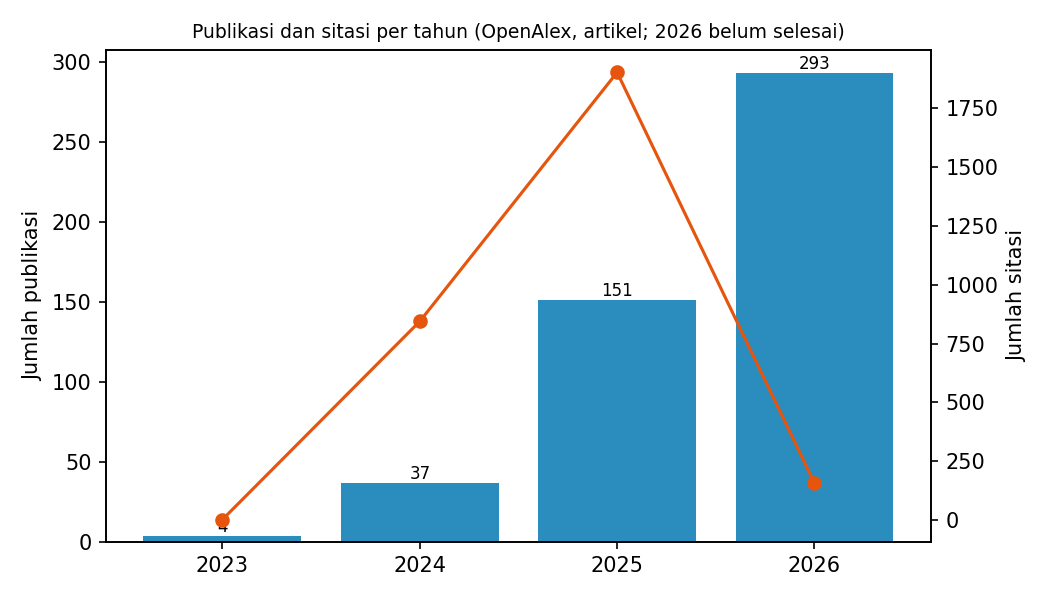
\includegraphics[width=0.75\textwidth]{figures/gambar1_tren_publikasi.png}
\caption{Publications and citations per year (OpenAlex, articles; 2026 is incomplete). \todo{redraw in the final journal style and in English}}
\label{fig:trend}
\end{figure}

The most cited documents are all about LLMs at the edge or small language models (Table~\ref{tab:A}); none concerns inventory or business operations. Authors are affiliated mostly with China (112 of the 485 articles have at least one Chinese affiliation), the United States (89), and India (43). Only 86 articles (18\%) have authors from two or more countries; the most frequent pairs are Hong Kong--China (15 articles), the United States--China (11), and China--Singapore (9). The dataset has 1{,}789 distinct author names, 3.92 authors per article on average, and only 14 names with three or more articles; name variants were not merged, so these figures are indicative.

\begin{table}[htbp]
\centering
\small
\caption{Top 10 document citation analysis}
\label{tab:A}
\begin{tabularx}{\textwidth}{|c|l|Y|c|}
\hline
\textbf{Rank} & \textbf{Author} & \textbf{Title} & \textbf{Citation} \\ \hline
1 & Ji Lin et al. & AWQ: Activation-aware Weight Quantization for On-Device LLM Compression and Acceleration & 273 \\ \hline
2 & Guanqiao Qu et al. & Mobile Edge Intelligence for Large Language Models: A Contemporary Survey & 240 \\ \hline
3 & Mingjin Zhang et al. & EdgeShard: Efficient LLM Inference via Collaborative Edge Computing & 227 \\ \hline
4 & Othmane Friha et al. & LLM-Based Edge Intelligence: A Comprehensive Survey on Architectures, Applications, Security... & 194 \\ \hline
5 & Yue Zheng et al. & A Review on Edge Large Language Models: Design, Execution, and Applications & 168 \\ \hline
6 & Fali Wang et al. & A Comprehensive Survey of Small Language Models in the Era of Large Language Models:... & 105 \\ \hline
7 & Zheng Lin et al. & Pushing Large Language Models to the 6G Edge: Vision, Challenges, and Opportunities & 92 \\ \hline
8 & Xinyuan Zhang et al. & Beyond the Cloud: Edge Inference for Generative Large Language Models in Wireless Networks & 77 \\ \hline
9 & Kailai Sun et al. & A review of AI edge devices and lightweight CNN and LLM deployment & 72 \\ \hline
10 & Rongjie Yi et al. & EdgeMoE: Empowering Sparse Large Language Models on Mobile Devices & 68 \\ \hline
\end{tabularx}
\par\vspace{2pt}{\normalsize Source: Authors' analysis of OpenAlex data.}
\end{table}


\subsection{Bibliographic coupling (RQ2)}
Of the 485 articles, 278 have reference data; 183 of them share at least two references with another article, forming 13 clusters of 43, 38, 35, 24, 14, 8, 5, 5, 3, 2, 2, 2, and 2 articles. Table~\ref{tab:B} lists the ten articles with the highest total link strength; they are surveys on edge and federated LLMs. Table~\ref{tab:C} summarises the clusters with at least five articles. \todo{label the clusters by revisiting representative articles (inductive interpretation) and replace the placeholders}

The five largest clusters consist almost entirely of articles from the on-device and edge block. The business-related articles form two small groups: one of eight articles whose representative items concern governed agentic process automation and reasoning applications, and one of five articles whose representative items concern LLMs for spare-parts demand forecasting and supply chain optimisation \todo{verify by reading the clusters' articles}. The business stream therefore exists in the reference network, but it is small and separate from the edge stream.

\begin{table}[htbp]
\centering
\small
\caption{Top 10 documents in the bibliographic coupling analysis}
\label{tab:B}
\begin{tabularx}{\textwidth}{cYcc}
\hline
\textbf{Rank} & \textbf{Publication} & \textbf{Citation} & \textbf{Total link strength} \\ \hline
1 & Wang et al. (2025), Empowering large language models to edge intelligence: A survey of edge... & 47 & 297 \\
2 & Friha et al. (2024), LLM-Based Edge Intelligence: A Comprehensive Survey on Architectures,... & 194 & 239 \\
3 & Piccialli et al. (2024), Federated and edge learning for large language models & 44 & 235 \\
4 & Sun et al. (2024), A review of AI edge devices and lightweight CNN and LLM deployment & 72 & 176 \\
5 & Zheng et al. (2025), A Review on Edge Large Language Models: Design, Execution, and Applications & 168 & 175 \\
6 & Xu et al. (2024), EdgeLLM: Fast On-Device LLM Inference With Speculative Decoding & 50 & 104 \\
7 & Yi et al. (2025), EdgeMoE: Empowering Sparse Large Language Models on Mobile Devices & 68 & 104 \\
8 & Qu et al. (2025), Mobile Edge Intelligence for Large Language Models: A Contemporary Survey & 240 & 80 \\
9 & Wang et al. (2025), Split Learning Based Cloud-Edge-End Collaborative Model Training in... & 5 & 77 \\
10 & Semerikov et al. (2025), Edge intelligence unleashed: a survey on deploying large language models in... & 20 & 75 \\ \hline
\end{tabularx}
\par\vspace{2pt}{\normalsize Source: Author interpretation based on VOSviewer analysis.}
\end{table}

\begin{table}[htbp]
\centering
\small
\caption{Summary of bibliographic coupling clusters (clusters with at least five documents).}
\label{tab:C}
\begin{tabularx}{\textwidth}{llrYY}
\toprule
\textbf{Cluster (colour)} & \textbf{Cluster label} & \textbf{No. of publications} & \textbf{Source block} & \textbf{Representative publications} \\
\midrule
1 (red) & \todo{to be labelled} & 43 & B: 39, A: 2, A+C: 1, C: 1 & Friha et al. (2024), LLM-Based Edge Intelligence: A Comprehensive Survey on Architectures,...; Piccialli et al. (2024), Federated and edge learning for large language models \\
2 (green) & \todo{to be labelled} & 38 & B: 37, C: 1 & Semerikov et al. (2025), Edge intelligence unleashed: a survey on deploying large language models in...; Jiang et al. (2026), Edge large language models: a comprehensive survey \\
3 (blue) & \todo{to be labelled} & 35 & B: 34, A: 1 & Wang et al. (2025), Empowering large language models to edge intelligence: A survey of edge...; Zheng et al. (2025), A Review on Edge Large Language Models: Design, Execution, and Applications \\
4 (yellow) & \todo{to be labelled} & 24 & B: 24 & Duan et al. (2026), SoK: Towards a user-centric, privacy-preserving, and reliable AI agent via...; Zhuang et al. (2026), Resource-Efficient LLM Customization on Mobile Devices Through Proxy Submodel... \\
5 (purple) & \todo{to be labelled} & 14 & B: 14 & Eccles et al. (2025), Mosaic: Composite projection pruning for resource-efficient LLMs; Luo et al. (2026), CALSI: Context-Aware Layer Skipping Inference for On-Device LLM Serving \\
6 (cyan) & \todo{to be labelled} & 8 & A: 4, B: 3, C: 1 & Bhattacharyya et al. (2026), The economics of accuracy for medical reasoning with large language models; Pacella et al. (2026), Governed Agentic Process Automation: A Floor-Safety Guarantee for... \\
7 (orange) & \todo{to be labelled} & 5 & B: 5 & Joshi et al. (2026), Securing the Cognitive Layer: A Survey on Security Threats, Defenses, and...; Jeong et al. (2025), On-Device Intent Reasoning for Smart Home Agents Via Ontology-Augmented sLLMs \\
8 (?) & \todo{to be labelled} & 5 & C: 3, A+C: 1, A: 1 & Nakhost et al. (2025), Full automation or just a copilot? A study of large language models on spare...; Hamdan et al. (2026), Evaluating large language models for complex supply chain optimisation: a focus... \\
\bottomrule
\end{tabularx}
\end{table}


\subsection{Co-citation (RQ2, foundations)}
Among 7{,}293 unique cited references, 346 were cited by at least three articles of the dataset (after removing eight artefacts, see Section~2.4), and they form four clusters of 133, 124, 85, and 4 references. The most strongly linked references (Table~\ref{tab:D}) are foundations of efficient LLM inference: LLaMA, structured pruning, quantisation, memory management for serving, and parameter-efficient fine-tuning. The three large clusters mix general LLM foundations with edge computing work, so they should not be labelled before the representative references are read. The fourth cluster has only four references, on generative AI in supply chain and operations management (Table~\ref{tab:E}). The business-related stream thus has no broad shared foundation in this dataset yet, but four references are a thin basis for a strong claim. \todo{verify the four references and read them before interpreting}

\begin{table}[htbp]
\centering
\small
\caption{Top 10 documents by co-citation total link strength (TLS); citations are counted within the dataset.}
\label{tab:D}
\begin{tabularx}{\textwidth}{rYrrr}
\toprule
\textbf{Rank} & \textbf{Document} & \textbf{Citations (within dataset)} & \textbf{TLS} & \textbf{Cluster} \\
\midrule
1 & Touvron (2023), LLaMA: Open and Efficient Foundation Language Models & 13 & 391 & 2 \\
2 & Ma (2023), LLM-Pruner: On the Structural Pruning of Large Language Models & 15 & 386 & 2 \\
3 & Shen (2024), Agile-Quant: Activation-Guided Quantization for Faster Inference of LLMs on the... & 10 & 379 & 3 \\
4 & Kwon (2023), Efficient Memory Management for Large Language Model Serving with PagedAttention & 19 & 369 & 2 \\
5 & B. (2020), Language Models are Few-Shot Learners & 16 & 358 & 2 \\
6 & Liu (2024), LLM-QAT: Data-Free Quantization Aware Training for Large Language Models & 10 & 332 & 2 \\
7 & Dettmers (2023), QLoRA: Efficient Finetuning of Quantized LLMs & 20 & 306 & 2 \\
8 & Alizadeh (2024), LLM in a flash: Efficient Large Language Model Inference with Limited Memory & 12 & 299 & 3 \\
9 & Vaswani (2025), Attention Is All You Need & 12 & 295 & 2 \\
10 & Ainslie (2023), GQA: Training Generalized Multi-Query Transformer Models from Multi-Head... & 9 & 295 & 2 \\
\bottomrule
\end{tabularx}
\end{table}

\begin{table}[htbp]
\centering
\footnotesize
\caption{Co-citation clusters on LLM research}
\label{tab:E}
\begin{tabularx}{\textwidth}{|l|Y|c|Y|}
\hline
\textbf{Cluster No and colour} & \textbf{Cluster label} & \textbf{Number of articles} & \textbf{Representative publication} \\ \hline
1 (red) & Edge LLM surveys, collaborative serving, and NLP benchmarks & 128 & Zhang (2024), EdgeShard: Efficient LLM Inference via Collaborative Edge Computing \\ \hline
2 (green) & Quantisation, pruning, and serving efficiency, with foundation models & 95 & Dettmers (2023), QLoRA: Efficient Finetuning of Quantized LLMs \\ \hline
3 (blue) & Mixed background: efficient inference, federated and parameter-efficient tuning, early applications & 58 & Alizadeh (2024), LLM in a flash: Efficient Large Language Model Inference with Limited Memory \\ \hline
4 (yellow) & General background: reasoning, edge computing visions, LLM agents, compression basics & 57 & Wei (2022), Chain-Of-Thought Prompting Elicits Reasoning in Large Language Models \\ \hline
5 (purple) & Generative AI in supply chain and operations management & 6 & Jackson (2024), Generative artificial intelligence in supply chain and operations management: a... \\ \hline
\end{tabularx}
\par\vspace{2pt}{\normalsize Source: Author interpretation based on VOSviewer analysis.}
\end{table}


\subsection{Co-word analysis (RQ3)}
Among 2{,}133 distinct keywords, 68 occurred at least eight times and formed three clusters of 24, 23, and 21 keywords (Tables~\ref{tab:F} and \ref{tab:G}, Figure~\ref{fig:coword}). Cluster~1 groups retrieval-augmented generation, multi-agent systems, agentic AI, LLM agents, inventory management, and demand forecasting; clusters 2 and 3 are about edge computing, model compression, and energy efficiency, and about small language models, on-device inference, and privacy. \todo{label clusters after reading representative articles}

\begin{figure}[htbp]
\centering
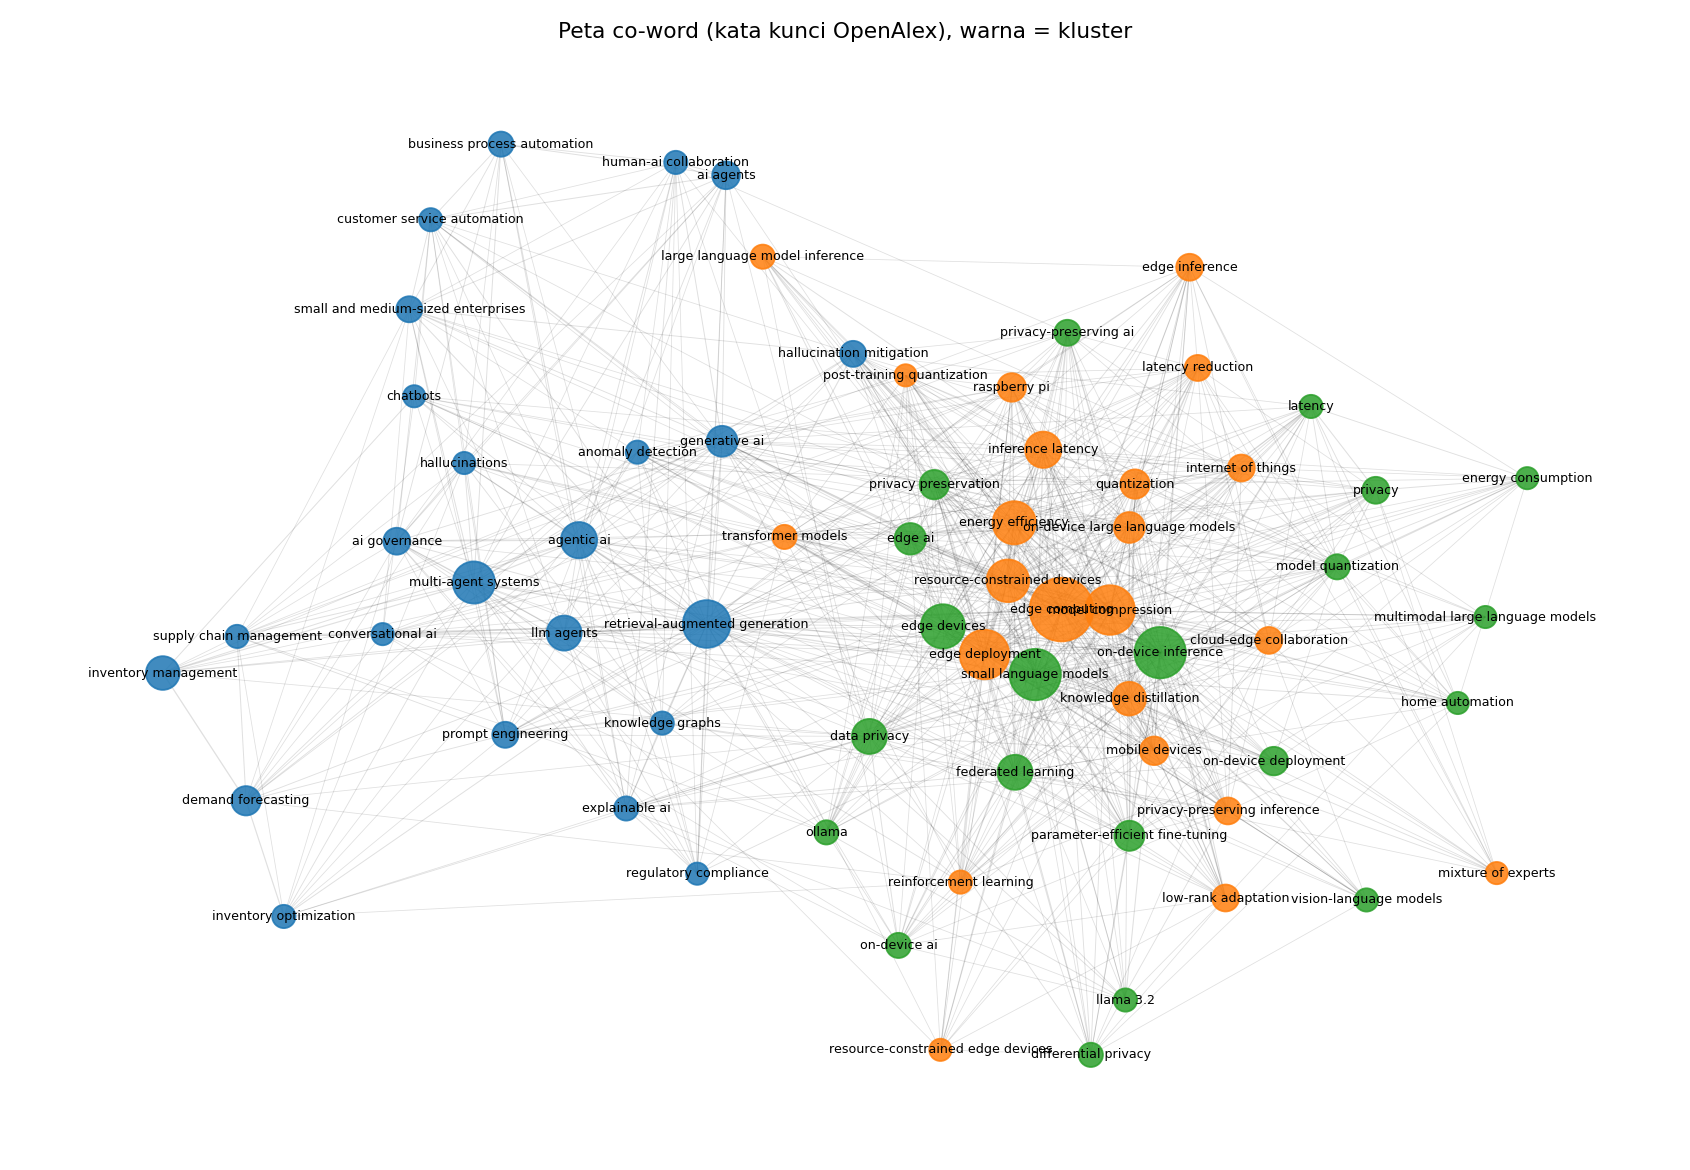
\includegraphics[width=\textwidth]{figures/peta_coword.png}
\caption{Co-word map (keywords assigned by OpenAlex, at least eight occurrences; colours show clusters). \todo{replace with the VOSviewer export with readable labels}}
\label{fig:coword}
\end{figure}

\begin{table}[htbp]
\centering
\small
\caption{Top 15 keywords in the co-occurrence of keywords analysis}
\label{tab:F}
\begin{tabularx}{\textwidth}{|c|Y|c|c|}
\hline
\textbf{Rank} & \textbf{Keyword} & \textbf{Occurrences} & \textbf{Total link strength} \\ \hline
1 & edge computing & 86 & 237 \\ \hline
2 & on-device inference & 55 & 136 \\ \hline
3 & small language models & 55 & 151 \\ \hline
4 & edge deployment & 51 & 127 \\ \hline
5 & model compression & 51 & 193 \\ \hline
6 & retrieval-augmented generation & 47 & 109 \\ \hline
7 & edge devices & 40 & 84 \\ \hline
8 & energy efficiency & 38 & 125 \\ \hline
9 & resource-constrained devices & 37 & 132 \\ \hline
10 & multi-agent systems & 36 & 73 \\ \hline
11 & agentic ai & 26 & 61 \\ \hline
12 & inference latency & 26 & 74 \\ \hline
13 & data privacy & 24 & 71 \\ \hline
14 & federated learning & 24 & 85 \\ \hline
15 & llm agents & 24 & 34 \\ \hline
\end{tabularx}
\par\vspace{2pt}{\normalsize Source: Author interpretation based on VOSviewer analysis.}
\end{table}

\begin{table}[htbp]
\centering
\footnotesize
\caption{Co-word analysis on LLM research}
\label{tab:G}
\begin{tabularx}{\textwidth}{|l|Y|c|Y|}
\hline
\textbf{Cluster No and colour} & \textbf{Cluster label} & \textbf{Number of keywords} & \textbf{Representative keywords} \\ \hline
1 (red) & Agentic AI and RAG for enterprise applications (with an inventory sub-theme) & 24 & retrieval-augmented generation, multi-agent systems, agentic ai, llm agents, inventory management, generative ai, demand forecasting, ai agents \\ \hline
2 (green) & Compression and optimisation for edge LLM deployment & 23 & edge computing, model compression, edge deployment, energy efficiency, resource-constrained devices, inference latency, knowledge distillation, on-device large language models \\ \hline
3 (blue) & Small language models and privacy-preserving on-device learning & 21 & on-device inference, small language models, edge devices, federated learning, data privacy, edge ai, parameter-efficient fine-tuning, privacy preservation \\ \hline
\end{tabularx}
\par\vspace{2pt}{\normalsize Source: Author interpretation based on VOSviewer analysis.}
\end{table}


\paragraph{Robustness.}
The agent and business keywords stayed in a cluster separate from the edge keywords in all 63 runs (minimum occurrences of 5, 8, and 12; 20 random seeds; and a greedy algorithm). However, modularity was low (0.18 to 0.26) and between 21\% and 54\% of the link weight crossed clusters. The clusters are therefore loosely separated groups with limited links, not disconnected fields.

\paragraph{Emerging topics.}
Colouring keywords by their mean publication year (Figure~\ref{fig:trendmap}) shows that business-oriented keywords such as small and medium-sized enterprises (mean year 2026.0), business process automation (2025.9), and hallucination mitigation (2025.9) are newer than inventory management and demand forecasting, which appear earlier in the dataset. On the edge side, local runtimes such as Ollama (2025.9) and mixture of experts (2025.9) are newer than the Internet of Things (2024.9) and privacy-preserving inference. The range of mean years is only about one year (2024.9 to 2026.0) and 2026 is incomplete, so we read this as an early trend, not as a firm finding. \todo{check the means against tren\_kata\_kunci.csv after the final dataset}

\begin{figure}[htbp]
\centering
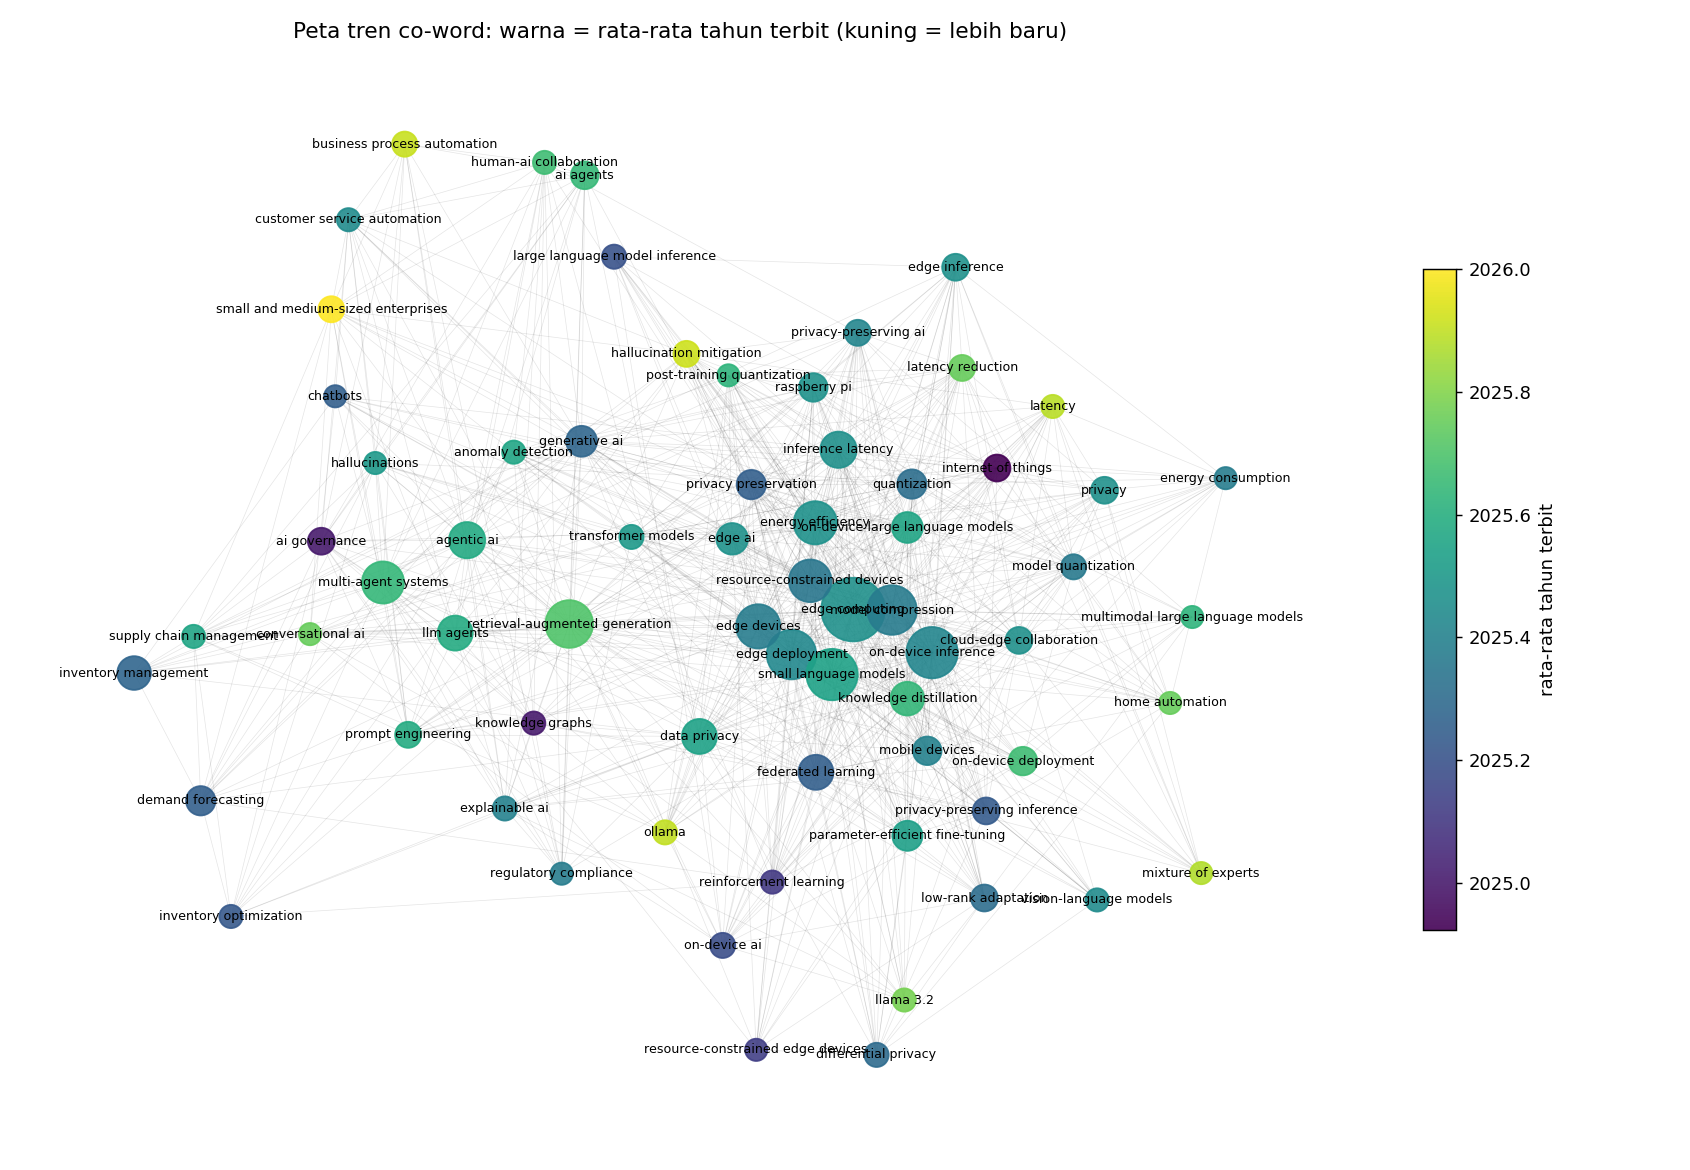
\includegraphics[width=\textwidth]{figures/peta_tren.png}
\caption{Co-word map coloured by mean publication year (yellow is more recent). \todo{replace with the VOSviewer overlay export}}
\label{fig:trendmap}
\end{figure}

\section{Implications}

% Diskusi sengaja ringkas: polanya sudah ada, tafsir teori dan perbandingan dengan review lain menunggu pembacaan dokumen inti.
\todo{Discussion: synthesise the three patterns (edge dominance, thin business stream, early shift towards agents and process automation); compare with earlier reviews; explain what the loose separation of clusters means. Write after the clusters are labelled.}

\subsection{Theoretical implications}
The maps suggest that research on LLMs for business operations has not yet built on the large body of work on efficient and local inference, although the two share concerns such as cost, latency, and privacy. \todo{derive claims from labelled clusters; do not state more than the data show}

\subsection{Managerial implications}
For small businesses that consider an LLM for inventory tasks, the evidence base in this dataset is small and mostly recent, so reported results should be treated with caution and tested on the business's own data. \todo{sharpen after reading the representative articles of the supply chain clusters}

\section{Limitations}
\label{sec:limitations}
The study has the following limitations, each linked to a direction for future work.
\begin{itemize}
  \item \textbf{One database.} We used OpenAlex, not Scopus or Web of Science. Coverage and metadata quality differ \todo{cite OpenAlex coverage studies after reading them, e.g.\ the reference coverage analysis by Culbert et al.\ (2025), found by search but not yet read}. Future work should repeat the search in Scopus or Web of Science and compare the maps.
  \item \textbf{Incomplete reference data.} Only 278 of 485 articles (57.3\%) have reference lists, which limits coupling and co-citation. Many missing lists come from journals that do not deposit references. A subset or a different source would help.
  \item \textbf{Partial year.} 2026 is incomplete, so yearly counts and trends for 2026 must not be read as a full year.
  \item \textbf{Search sensitivity.} Search is limited to titles and abstracts, and variations of the keywords were not tested. A sensitivity check with alternative terms is needed.
  \item \textbf{Model-assisted screening.} Screening used language models; \todo{report the manual validation and its agreement}. Low-confidence decisions remain.
  \item \textbf{Keywords.} Keywords come from OpenAlex's automatic assignment, not from the authors.
  \item \textbf{Cluster labels and layout.} Cluster membership depends on the algorithm and thresholds; the robustness check shows stable membership but low modularity.
\end{itemize}

\section{Future research avenues}
\todo{Make these specific enough to become study designs. Candidates: (i) a Scopus/Web of Science replication; (ii) a content analysis of the supply chain and inventory articles to test how far results transfer to small businesses; (iii) empirical studies of agent-based LLM systems for inventory tasks that run on local or in-browser models, evaluated on real transaction data.}

\section{Conclusion}
\todo{Close with the contribution, not only a summary. Draft after the discussion is written.}


\section*{Declarations}
\noindent\textbf{Use of AI tools.} Claude (Anthropic) assisted with record screening (title and abstract), data processing scripts, and drafting of the text. The author reviewed the outputs \todo{state the extent of manual validation once the sample check is complete} and takes responsibility for the content. \todo{check the target journal's policy on AI disclosure}

\noindent\textbf{Data and code availability.} Search strings, scripts, and the screened dataset are in the accompanying repository (folder \texttt{analysis}). Records come from OpenAlex. \todo{add repository URL or archive DOI}

\bibliographystyle{apalike}
\bibliography{refs}

\end{document}
